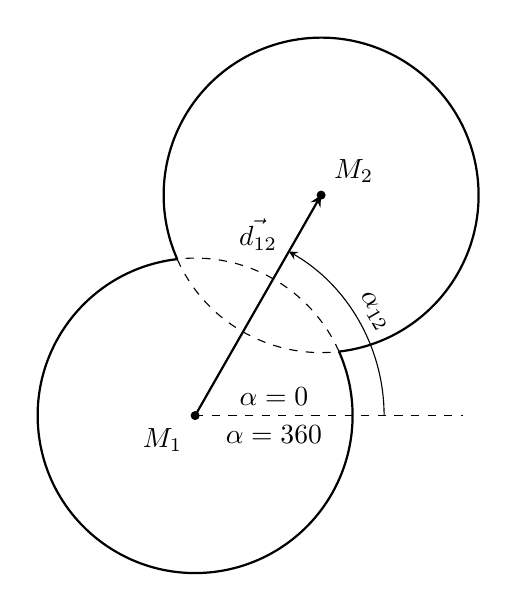
\begin{tikzpicture}[
    scale=2,
    >=stealth,
    point/.style = {draw, circle,  fill = black, inner sep = 1pt},
    dot/.style   = {draw, circle,  fill = black, inner sep = .2pt},
  ]
  
	\coordinate (R1) at (1,1); % Mittelpunkt des ersten Kreises
	\coordinate (R2) at (1.8,2.4); % Mittelpunkt des zweiten Kreises
	
	% Kreismittelpunkte
	\node (M1) at (R1) [point, label = {below left:$M_1$}]{};
	\node (M2) at (R2) [point, label = {above right:$M_2$}]{};
	
	% Bögen
	% C1
	\draw[thick] (R1) ++(96.53:1) arc (96.53:383.98:1);
	\draw[dashed] (R1) ++(23.98:1) arc (23.98:96.53:1);
	
	% C2
	\draw[thick] (R2) ++(276.53:1) arc (276.53:563.98:1);
	\draw[dashed] (R2) ++(203.98:1) arc (203.98:276.53:1);
	
	%\draw[->] (R1) ++(100:1.2) arc (100:160:1.2) node[midway, sloped, above]{$l$};
	
	% Abstandsvektor d12
	\draw[thick,->] (R1) -- (R2);
	\node at (1.4,2.15) {$\vec{d_{12}}$};
	
	% Hilfslinie zur Sichtbarmachung der 0°/360° Grenze
	\draw[dashed] (R1) -- (2.7,1);
	\node [below] at (1.5,1) {$\alpha = \ang{360}$};
	\node [above] at (1.5,1) {$\alpha = \ang{0}$};
	
	% Winkelpfeil
	\draw[->] (R1) ++(0:1.2) arc (0:60.26:1.2) node[midway, sloped, above]{$\alpha_{12}$};
	
\end{tikzpicture}